
\documentclass[tikz]{standalone}
%\usetikzlibrary{shadows}
%\usetikzlibrary{backgrounds}
\usetikzlibrary{calc,positioning}

\begin{document}
\begin{tikzpicture}%[show background rectangle, background rectangle/.style={fill=black}]
	%variables
	\def\roadlength{30}
	\def\lanewidth{3.5}
	\def\dashedon{0.6}  % /!\ in cm
	\def\dashedoff{1.2} % /!\ in cm
	\def\linewidth{0.15} % /!\ in cm
	\def\vehiclelength{6}


	%colors
	\definecolor{dark-gray}{gray}{0.1}
	\definecolor{trust-yellow}{rgb}{255,192,0}
	
	% asphalt
	\node[rectangle,fill=dark-gray!60, anchor = north west, minimum width=\roadlength cm,minimum height=30 + 3*\lanewidth cm] (asphalt)  at (0,20 + 3*\lanewidth cm){};
	
	% ground painting
  	\draw [white, line width=\linewidth cm](0,0) -- (\roadlength,0); 
	\draw [white, dashed,line width=\linewidth cm, dash pattern=on \dashedon cm off \dashedoff cm](0,\lanewidth-0.5*\linewidth) -- (\roadlength,\lanewidth); 
	\draw [white, dashed,line width=\linewidth cm, dash pattern=on \dashedon cm off \dashedoff cm](0,2*\lanewidth-0.5*\linewidth) -- (\roadlength,2*\lanewidth+\linewidth); 
  	\draw [white, line width=\linewidth cm](0,3*\lanewidth+2*\linewidth) -- (\roadlength,3*\lanewidth+2*\linewidth);
	
	
	%%% vehicles
	
	% lane 1
	
	\node (v11) at (-8 + 0.5*\roadlength,1*\lanewidth - 0.5*\lanewidth) {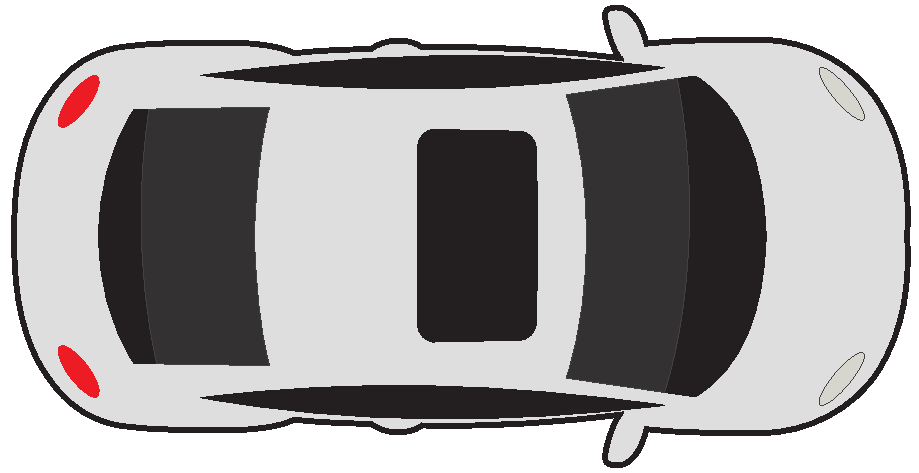
\includegraphics[width=\vehiclelength cm]{src/simple_vehicle.pdf}};
	
	% lane 2
	
	% current vehicle (highlighted with a cyan rectangle arround it)
	\node[rectangle,draw=cyan, line width=1mm, inner sep=0pt] (v2i) at (-5+0.5*\roadlength,2*\lanewidth - 0.5*\lanewidth) {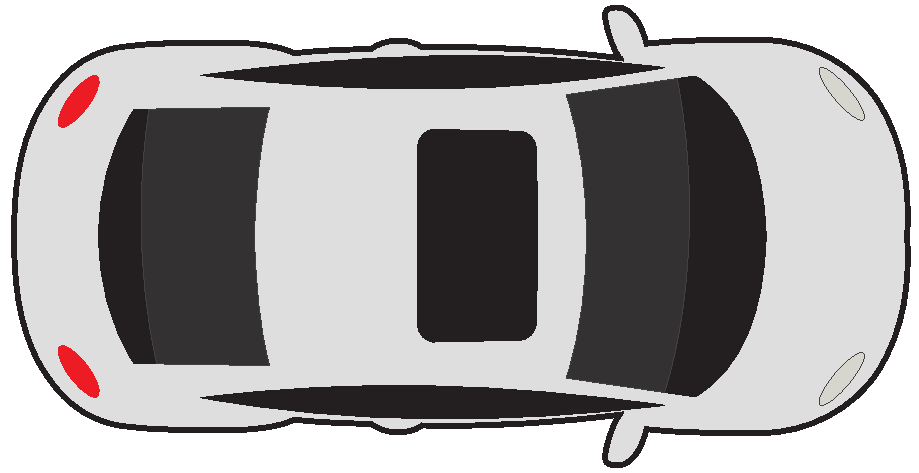
\includegraphics[width=\vehiclelength cm]{src/simple_vehicle.pdf}};
	
	\node (v21) at (7 + 0.5*\roadlength,2*\lanewidth - 0.5*\lanewidth) {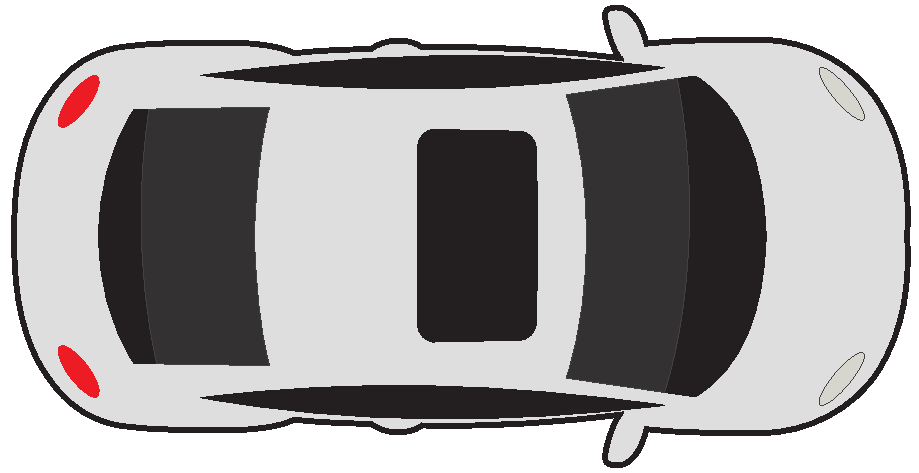
\includegraphics[width=\vehiclelength cm]{src/simple_vehicle.pdf}};
	
	%lane 3
	
	\node (v31) at (5 + 0.5*\roadlength,3*\lanewidth - 0.5*\lanewidth) {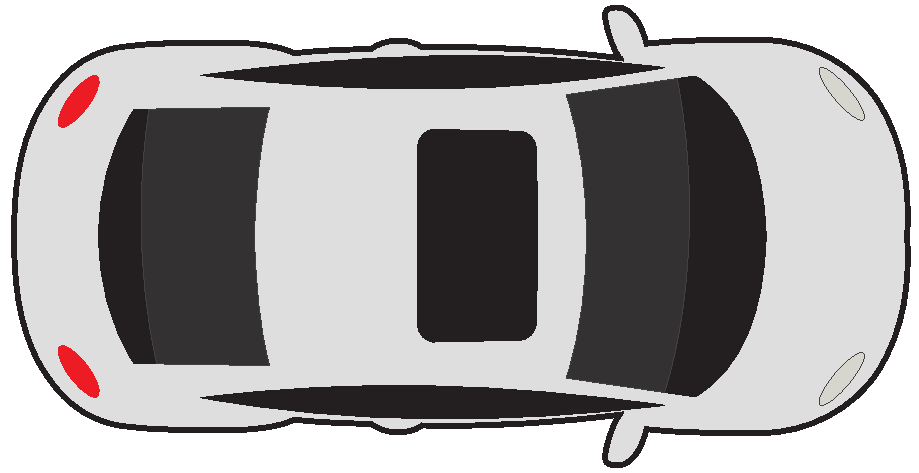
\includegraphics[width=\vehiclelength cm]{src/simple_vehicle.pdf}};

	\node[scale=1.5,rectangle,fill=violet, draw=black, minimum width=2cm,minimum height=1cm, line width=0.5mm, text=white] (rsu) at (0.5*\roadlength,- 1) {\Huge RSU};
	
	
	%perception
	%\draw [>=latex,line width=4pt,->,red] (v2i.east) -- (v21.west);
	
	\path[>=latex,line width=2pt,<->,green] (v21.center) edge [bend left=20] (v2i);
	\path[>=latex,line width=2pt,<->,green] (v31.center) edge [bend left=-20] (v2i);
	
	\path[>=latex,line width=2pt,<->,violet] (rsu) edge [bend left=-20] (v2i);
	
	\tikzstyle{legend}=[scale=2, anchor=west, align = flush left]
	
	%% percpetion range
	
	%%% Legend
	%% column 1
	\node[legend,rectangle,draw=cyan, line width=1mm, inner sep=0pt] at (0.01, -3) {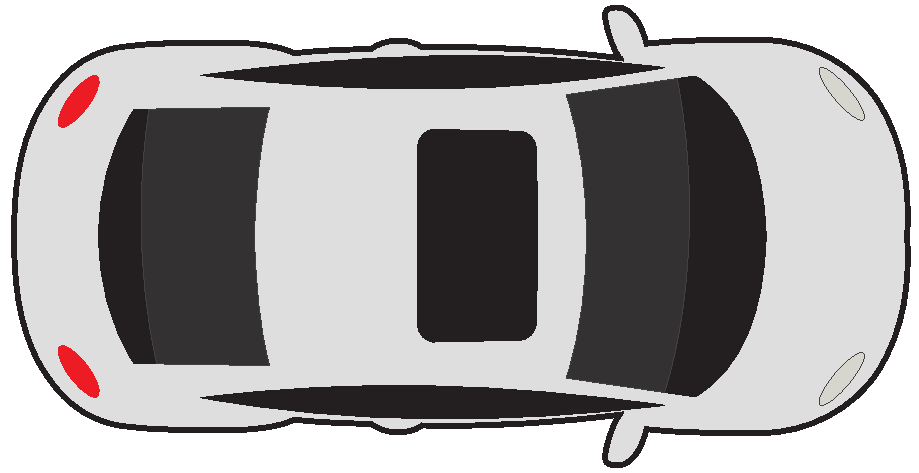
\includegraphics[width=1.5cm]{src/simple_vehicle.pdf}};
	
	
	\draw [>=latex,line width=2pt,<->,green] (0.05, -5) -- (0.1*\roadlength, -5);
	\draw [>=latex,line width=2pt,<->,violet] (0.52*\roadlength, -5) -- (0.58*\roadlength, -5);
	
	
	\node[legend] at (0.11*\roadlength, -3) {\large Regular vehicle};
		
	\node[legend] at (0.11*\roadlength, -5) {\large Information exchange -- V2V};
	\node[legend] (legend21) at (0.6*\roadlength, -5) {\large V2I/I2V};

\end{tikzpicture}
\end{document}